\chapter{Semissupervisão no Aprendizado em Fluxo de Dados} \label{ChSemi}

%Tendo em conta os aspectos envolvidos no aprendizado em FD e o recente crescimento de esforços para encontrar soluções capazes de lidar com os desafios encontrados nesta variedade de domínios, evidenciado na \autoref{chConceitos:FD}, julga-se interessante a investigação mais aprofundada das diversas propostas existentes na literatura para aprendizado em FD.

%As propostas de técnicas para aprendizado em FD são, na maioria das vezes, adaptações de técnicas de aprendizado clássico para lidar com um ou mais desafios encontrados em domínios de FD, e.g.: a necessidade de processar os dados logo que chegam, seja de forma \emph{online} (exemplo a exemplo) ou considerando partes do conjunto de exemplos (processamento de \emph{chunks}); a adaptação do modelo geral que representa o FD e a otimização de suas estruturas; a detecção e tratamento de desvios de conceito.

%Algumas técnicas de aprendizado incremental foram desenvolvidas para domínios específicos ou com foco em conjuntos de dados que, embora volumosos, não apresentam características de FD, como, por exemplo, questões de desvio de conceito. Ainda que o foco principal das propostas não seja o aprendizado em FD, certas abordagens podem ser aplicadas neste contexto, porém com algumas ressalvas, já que não possuem mecanismos para lidar com um ou outro aspecto intrínseco aos domínios FD.

%Este capítulo apresenta discussão sobre uma revisão bibliográfica de abordagens para aprendizado em FD organizadas de acordo com as suas principais características, desenvolvidas especificamente com este intuito ou não. As técnicas colocadas neste capítulo consideram a abordagem de aprendizado por exemplos, em que o processo de aprendizagem tem seu foco nas instâncias de um único FD.

%\section{Técnicas de Classificação em Fluxos de Dados}

%No caso em que o FD envolve dados rotulados, o aprendizado pode ser feito por meio de técnicas supervisionadas. Encontra-se na literatura um volume significativo de trabalhos que utilizam a indução de modelos baseados em árvores. Outros trabalhos abordam o assunto propondo a criação de modelos híbridos utilizando conceitos \emph{fuzzy}. Outra abordagem bastante explorada nesse contexto é a integração de múltiplos modelos. A seguir, alguns trabalhos representativos dessa categoria são apresentados.
%%\undecided{\subsection{Aprendizado Supervisionado em FD baseado em Árvores}}
%
%A indução de árvores de decisão é uma forma de aprendizado supervisionado amplamente utilizada e tem sido bastante explorada dentro do contexto de FDs. Muitas das propostas envolvendo árvores de decisão utilizam ideias gerais das AH, apresentadas na \autoref{chConceitos:FD:HoeffdingTrees}.
%
%O algoritmo \emph{Incremental Extremely Random Forest} \cite{Wang2009} considera o aprendizado, feito por árvore de decisão baseada em AH, em FDs com baixo volume de exemplos, mas em domínios onde seja necessária a adaptação do modelo geral de classificação.
%
%A \emph{Very Fast Decision Tree} (VFDT) \cite{Domingos2000}, uma proposta de aprendizado incremental baseada em AH, serviu de fundamento para outros métodos.  A abordagem utiliza limiares de Hoeffding para garantir que a saída de suas árvores seja o mais próxima de um classificador convencional, que aprende a partir de conjuntos estáticos.
%
%Uma das propostas que utiliza VFDT é a \emph{Concept-adapting Very Fast Decision Tree} (CVFDT) \cite{Hulten2001}, que tem como foco a detecção e adaptação a desvios de conceito em FDs. \citeonline{Liu2009} apresentam uma proposta de um mecanismo para integração de ambiguidades à CVFDT, modificando a divisão de nós pela exploração de múltiplas opções. A técnica visa garantir que o conhecimento mais novo seja utilizado na divisão dos nós, mas também é capaz de reaprender conceitos ressurgentes.
%
%\citeonline{Tsai2009} apresentam uma proposta diferenciada para mineração de regras de desvios de conceitos, buscando encontrar a regra que governa o desvio identificado. A mineração de regras de conceito é feita pelo algoritmo CDR-Tree, que considera dois blocos de dados de um FD que dizem respeito aos mesmos indivíduos em tempos distintos. A partir dos exemplos de cada bloco, o algoritmo forma pares que serão utilizados para a construção de uma árvore de decisão tradicional. As regras de desvio de conceito são mineradas a partir da árvore construída com os pares de exemplos velhos (bloco de dados no tempo $\delta$) e novos (bloco de dados no tempo $\delta + t$). No mesmo trabalho são propostas estratégias para diminuir a complexidade das regras de desvio de conceito mineradas.
%
%%\undecided{\subsection{Aprendizado Supervisionado em FD que utilizam Fuzzy}}
%
%Dentro do conjunto de abordagens para aprendizado supervisionado em FD também encontramos alguns métodos híbridos que se utilizam de conceitos \emph{fuzzy}.
%
%\emph{Fuzzy Pattern Trees} \cite{Huang2008} são árvores induzidas por processo diferenciado, utilizando operadores de agregação distintos de árvores de decisão \emph{fuzzy} tradicionais, podendo gerar regras que utilizam t-conormas (OU) além de t-normas (E). A fim de ilustrar a diferença entre as estruturas, a \autoref{Fig:FDTvsFPT} traz as árvores de decisão construídas a partir de um mesmo pequeno conjunto de dados exemplo utilizando um algoritmo tradicional de árvore de decisão \emph{fuzzy} (\autoref{Fig:FDTvsFPT_FDT}) e o algoritmo proposto para a construção de \emph{Fuzzy Pattern Trees} (\autoref{Fig:FDTvsFPT_FPT}).
%
%\begin{figure}[!htb]
%        \centering
%        \begin{subfigure}[t]{0.3\textwidth}
%                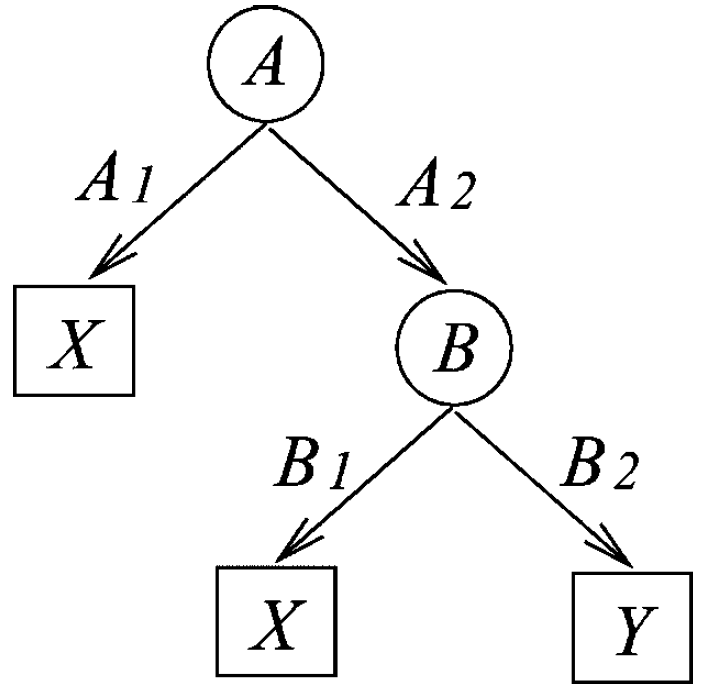
\includegraphics[width=\textwidth]{figures/FDTvsFPT_FDT}
%                \caption{Árvore de decisão \emph{Fuzzy}}
%                \label{Fig:FDTvsFPT_FDT}
%        \end{subfigure}%
%        \hspace{6em} %add desired spacing between images, e. g. ~, \quad, \qquad, \hfill etc.
%          %(or a blank line to force the subfigure onto a new line)
%        \begin{subfigure}[t]{0.3\textwidth}
%                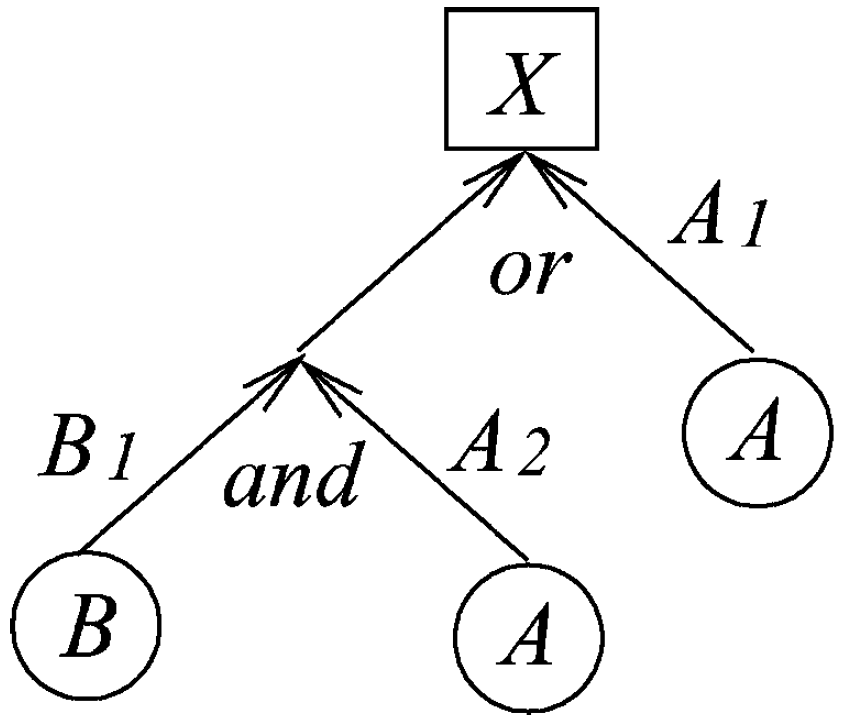
\includegraphics[width=\textwidth]{figures/FDTvsFPT_FPT}
%                \caption{\emph{Fuzzy Pattern Tree}}
%                \label{Fig:FDTvsFPT_FPT}
%        \end{subfigure}
%        \caption{Exemplos de árvores construídas a partir de um mesmo conjunto de exemplos \cite{Huang2008}}\label{Fig:FDTvsFPT}
%\end{figure}
%
%A proposta apresentada em \cite{Shaker2013} é um método de classificação adaptativo baseado na indução de \emph{Fuzzy Pattern Trees}. Esta proposta implementa um mecanismo de adaptação que identifica, de forma preditiva, possíveis mudanças locais no modelo atual. A ideia básica do método é manter um conjunto de \emph{Fuzzy Pattern Trees} composto pelo modelo atual (ativo) e um conjunto de modelos vizinhos. A predição é realizada pelo modelo ativo, enquanto os modelos vizinhos funcionam como adaptações antecipadas. Os modelos vizinhos são mantidos até que a performance do modelo ativo tenha queda significativa, causada, por exemplo, por um desvio de conceito. Neste momento, o modelo atual é substituído pelo modelo vizinho mais adequado.
%
%\citeonline{Wang2013} expõem a proposta de um \emph{framework} geral para a utilização de pesos \emph{fuzzy} para cada exemplo do FD. De forma incremental, conforme a chegada de novos exemplos, o cálculo da pertinência, baseado na informação de rótulo, é efetuado, levando em conta as pertinências já calculados para exemplos antigos. O cálculo de distância proposto e utilizado no trabalho, que é baseado na descoberta de centróides de classe e distância entre pares de exemplos, pode colaborar para a identificação de possíveis \emph{outliers}. A priori, o \emph{framework} pode ser utilizado em conjunto com qualquer algoritmo de classificação que faça uso da informação obtida na forma de pesos. Os autores optaram por vincular, de forma direta, um algoritmo baseado em redes neurais, o \emph{Passive-Agressive} (PA) \cite{Crammer2006}, constituindo a técnica neuro-\emph{fuzzy} \cite{Jang1997} chamada de \emph{Fuzzy Passive-Agressive}.
%
%%\undecided{\subsection{Aprendizado Supervisionado em FD baseado em \emph{Ensemble} de Classificadores}}
%
%A ideia da construção de um modelo preditivo pela integração de múltiplos modelos \cite{Witten2005,Rokach2010} também pode ser encontrada no aprendizado em FD. Abordagens que se utilizam deste sistema serão tratadas, doravante, pelo termo geral \emph{Ensemble} de Classificadores (EC).
%
%\citeonline{Tsymbal2008} propõe uma técnica de integração dinâmica de EC para auxiliar no trabalho de identificação e tratamento de desvios de conceito, onde cada classificador recebe um peso proporcional a sua acurácia local. Para a classificação final, o melhor classificador base, quando houver, é selecionado ou é realizada uma votação ponderada entre os classificadores.
%
%Desvios de conceitos e contexto é o foco no trabalho de \citeonline{Gomes2011}. A proposta baseada em EC realiza a detecção de mudanças de conceito e, dinamicamente, adiciona e remove classificadores ponderados de acordo com o que foi identificado. Conceitos estáveis são detectados por método baseado na taxa de erro do processo de aprendizado. A informação de contexto é utilizada na adaptação a conceitos recorrentes (ou ressurgentes) e no gerenciamento de conhecimento aprendido previamente.
%
%%\undecided{\subsection{Other ?}}
%
%A dificuldade de classificação de instâncias incompletas também é uma preocupação quando tratamos de aprendizado em FD. A maior parte das abordagens assume que todos os exemplos do FD possuem valores para um determinado conjunto de atributos, no entanto existem esforços \cite{MillanGiraldo2011} para que os exemplos sem um ou mais atributos possam ser aproveitados no processo de aprendizagem. 
%
%Pesquisadores têm investido na área de classificação em FD, porém é importante ressaltar que nem sempre existem rótulos disponíveis para realizar esse tipo de tarefa de aprendizado e a rotulação manual dos exemplos de um FD é inviável considerando seu tamanho potencialmente infinito. A próxima seção descreve técnicas de agrupamento em FD. 

%\section{Técnicas de Aprendizado Semissupervisionado em Fluxos de Dados}

A busca por melhores resultados no aprendizado em FD impulsionou o desenvolvimento de técnicas semissupervisionadas para trabalhar neste contexto. As abordagens de aprendizado semissupervisionado para conjuntos estáticos, juntamente com as abordagens de aprendizado supervisionado e não supervisionado em FD servem de inspiração para as propostas descritas nas próximas seções.

\section{Classificação Semissupervisionada em FD}

As técnicas de aprendizado semissupervisionado baseadas em classificadores assumem que o conjunto de dados é parcialmente rotulado. No caso desse tipo de aprendizado em FD, a parte rotulada dos exemplos pode ser apenas um pequeno conjunto que irá gerar o modelo inicial de classificação ou é possível encontrar exemplos rotulados no próprio fluxo.

Considerando essas duas situações de disponibilidade de rótulos, podem ser encontradas na literatura propostas baseadas em diferentes métodos de classificação, por exemplo: redes neurais \cite{Leite2010,Astudillo2011,Astudillo2013,Bouguelia2013,Kasabov2013}, baseada em grafos \cite{Tiwari2010,Bertini2012,Bertini2013}, competição de partículas \cite{Breve2012,Breve2013}, SVM \cite{Frandina2013}, entre outros \cite{Pan2007,FdezRiverola2007,DeSilva2011}.

Uma proposta \cite{Liang2012} baseada em CVFDT considera que o FD possui rótulo positivo e os dados incertos são não rotulados, realizando o aprendizado de forma semissupervisionada.

Técnicas baseadas em \emph{ensemble} de classificadores também são populares no aprendizado semissupervisionado em FD. \citeonline{Kholghi2011} apresentam uma proposta para um \emph{framework} que combina semissupervisão por meio de \emph{Active Learning} \cite{Settles2010} e a consideração da influência de exemplos não rotulados a fim de melhorar a performance de aprendizagem. Um modelo é construído para predição de rótulos de exemplo futuros com alto valor de acurácia. Esse modelo de predição é baseado em um \emph{ensemble} de classificadores construídos a partir de \emph{chunks} de exemplos do FD. Esta é uma das primeiras tentativas de incorporação de \emph{Active Learning} semissupervisionado em FD.

\section{Agrupamento Semissupervisionado em FD}

No aprendizado semissupervisionado baseado em agrupamento, considera-se conhecimento prévio durante o processo de agrupamento para melhorar o aprendizado. Esta informação pode estar disponível em diferentes formas, por exemplo rótulos para parte do FD, restrições entre pares de exemplos, informações estatísticas sobre a distribuição dos exemplos.

Quando há uma pequena quantidade de exemplos rotulados disponíveis, estes podem ser utilizados como sementes que contribuirão para guiar o algoritmo de agrupamento. O modelo de \emph{flocking} serve de inspiração para a adaptação de um algoritmo de agrupamento para aprendizado em FD \cite{Bruneau2009}, utilizando um pequeno conjunto de dados rotulados como informação para um operador de divisão de um grupo de exemplos, que permite a adaptação do agrupamento a mudanças no FD.

Uma técnica de agrupamento semissupervisionado baseada em AP \cite{Shi2009} utiliza informação prévia na forma de rótulos no ajuste da matriz de similaridade do modelo produzido e promove um estudo para ampliar o conjunto de dados rotulados. Baseado em \emph{Fuzzy Pattern Matching} \cite{Cayrol1982,Dubois1988}, o método proposto em \cite{Mouchaweh2010} tem o objetivo de aprender funções de pertinência com um conjunto de exemplos rotulados inicial limitado. A função de pertinência das classes é aprendida e atualizada, de acordo com a chegada de novos exemplos com rótulos.

O algoritmo \emph{Compound Gaussian Mixture Model} \cite{Gao2010}, baseado no agrupamento \emph{Gaussian Mixture Model}, utiliza amostra de dados rotulados em uma fase que aplica uma extensão do algoritmo \emph{Expectation Maximization} \cite{Zhou2007} para melhorar o agrupamento. A técnica \emph{Growing Type-2 Fuzzy Classifier} \cite{Bouchachia2014} utiliza uma versão \emph{online} do agrupamento \emph{Gaussian Mixture Model} para gerar partições \emph{fuzzy} tipo-2 \cite{Mendel2002} para construir regras de classificação, empregando conjunto parcialmente rotulado no aprendizado. Esta técnica possui mecanismos para aprendizado em FD.

\citeonline{Atwa2014} propõem um algoritmo de agrupamento semissupervisionado que extende o AP para lidar com FD. Um conjunto de instâncias rotuladas é incorporado para detecção de mudança, que requer a atualização do modelo o mais rápido possível. 

Em um contexto de FD com multirrótulos, o \emph{Hierarchical Semi-supervised Impurity based Subspace Clustering} \cite{Ahmed2010} captura a correlação implícita existente entre cada par de rótulos de classe.

Técnicas que utilizam informação na forma de restrições podem obtê-las a partir de exemplos rotulados, mas também pode ser um conhecimento pré-existente nesse formato. O \emph{C-DenStream} \cite{Ruiz2009} é uma técnica baseada no algoritmo \emph{DenStream} adaptado para a utilização o conceito de restrições entre pares de exemplos estendido para FD. O \emph{C-DenStream} foi uma das primeiras extensões do paradigma de aprendizado por agrupamento semissupervisionado estático para FD e, embora traga ganhos nesse contexto, ainda possui as limitações do \emph{DenStream}. 

\citeonline{Halkidi2012} utiliza, além do FD, um fluxo contínuo de restrições, introduzindo o conceito de multigrupos (regiões densas e sobrepostas) e implementa mecanismo para identificação de \emph{outlier}. \citeonline{Sirampuj2013} \label{chRevisao:Sirampuj2013} propõem um algoritmo para agrupamento em FD também com uso de conhecimento prévio na forma de restrições. A técnica, que é uma extensão do \emph{E-Stream} \cite{Udommanetanakit2007} possui mecanismos para lidar com restrições que mudam de acordo com o tempo (técnica de esquecimento).

\citeonline{Cheng2011} desenvolvem um \emph{framework} para análise de agrupamento de textos e desenvolvimento de um novo modelo de agrupamento semissupervisionado, capaz de lidar com informação prévia na forma de restrições entre pares de exemplos e rótulos de maneira simultânea.

Uma proposta de método para agrupamento em FD incertos (domínios onde há ruído e dados incompletos) \cite{Aggarwal2008} utiliza um modelo geral de incerteza, no qual assume-se que algumas estatísticas de incerteza estão disponíveis. 

\section{Aprendizado Semissupervisionado Híbrido em FD}

É possível identificar dentro do aprendizado semissupervisionado algumas abordagens híbridas, ou seja, inspiradas em métodos de agrupamento e classificação trabalhando em conjunto para melhorar o aprendizado.

\citeonline{Wu2009} apresentam um método semissupervisionado para a construção de um rastreador de tópicos (\emph{topical crawler}), aplicando um agrupamento $k$-\emph{means} com restrições entre pares para detectar novas amostras de páginas enviadas a um classificador de páginas e preditor de links para atualização de modelos aprendidos.

A proposta de \citeonline{Borchani2011} é a combinação do método de \cite{Dasu2006} adaptado em um algoritmo de agrupamento para aprendizado semissupervisionado. O algoritmo de agrupamento é utilizado para atualização do modelo quando ocorre desvio de conceito.

Técnicas baseadas em AH podem utilizar métodos de agrupamento para divisão e rotulação em suas folhas. \citeonline{Li2012} estende trabalho anterior \cite{Li2010} e propõem um algoritmo de classificação semissupervisionada em FD, utilizando uma árvore de decisão como modelo de classificação. Para o crescimento da árvore, utiliza-se de um algoritmo de agrupamento baseado no $k$-\emph{means} para a produção de grupos de conceito e rotulação automática de dados não rotulados. Potenciais desvios de conceito são identificados e conceitos recorrentes são mantidos. Uma técnica semelhante considera informação prévia na forma de rótulos e aplica uma versão semissupervisionada do algoritmo de agrupamento $k$-\emph{modes} para produzir grupos de conceito \cite{Li2010a,wu2012}.

\emph{Clustering Feature Decision Tree} \cite{Xu2011} realiza a construção de uma árvore de decisão a partir de FD parcialmente rotulados, aplicando algoritmo de agrupamento para gerar um vetor de atributos de grupos, sumários estatísticos que serão usados para indução da árvore de decisão. Os vetores de grupos também são empregados na classificação de exemplos nas folhas da árvore.

\citeonline{Zhang2009} propõem um \emph{framework} para construção de modelos a partir de FD com exemplos rotulados e não rotulados. Para a construção do modelo, os dados do FD são associados a quatro categorias distintas, cada qual correspondendo à situação de desvio de conceito, podendo existir ou não nos exemplos rotulados e não rotulados. Em seguida, é aplicado método de aprendizado SVM semissupervisionado baseado no $k$-\emph{means}.

A técnica \emph{Concurrent Semi-supervised Learning of Data Streams} \cite{Nguyen2011,Nguyen2013} aplica o potencial de aprendizado semissupervisionado concorrente, onde um modelo de agrupamento e um de classificação são construídos de forma simultânea e colaborativa, fazendo uso de um pequeno conjunto de exemplos rotulados encontrados em um FD.

Outras propostas utilizam aprendizado semissupervisionado com objetivo de apenas estender o conjunto de exemplos rotulados e, então, aplicar método de aprendizado supervisionado com mecanismos disponíveis para lidar com as particularidades de FD. \citeonline{Wu2006} coloca a proposta de um algoritmo de aprendizado semissupervisionado baseado em treinamento por agrupamento, para seleção de exemplos confiáveis a serem rotulados e utilizados no retreinamento de um classificador. A técnica proposta por \cite{Yu2009} aplica um algoritmo de agrupamento semissupervisionado aos exemplos parcialmente rotulados do FD na tentativa de estender o conjunto de exemplos rotulados, utilizando-os para atualização de um modelo supervisionado que conta com mecanismos de esquecimento.

O \emph{framework} \emph{COMPOSE} \cite{Dyer2014} aprende desvios de conceitos em ambiente de FD onde há apenas um conjunto inicial de dados rotulados e, após a inicialização, apenas dados não rotulados. O \emph{COMPOSE} segue três passos:
\begin{enumerate*}[label=\itshape\arabic*\upshape)]
\item combinação dos dados rotulados iniciais aos dados não rotulados atuais para treinar um classificador semissupervisionado e rotular de forma automática o conjunto de dados;
\item para cada classe, construção de formas que englobam os exemplos, representando a distribuição atual da classe;
\item compactação das formas e extração de instâncias representantes (\emph{core supports}), que servirão como conjunto rotulado inicial para os próximos novos dados não rotulados
\end{enumerate*}.

\section{\emph{Ensemble} de Modelos para Aprendizado Semissupervisionado em FD}

Algumas propostas para aprendizado semissupervisionado em FD tem a intenção de aproveitar da construção de diversos modelos trabalhando em conjunto para melhorar a representação dos exemplos do FD.

O trabalho apresentado em \cite{Zhang2012} é uma adaptação do trabalho \cite{Zhang2009}, onde para cada categoria de exemplo de treinamento é construído um modelo distinto para classificação, baseado em SVM. Em \cite{Zhang2014a} os modelos base para o \emph{ensemble} são construídos por método de aprendizado semissupervisionado, utilizando conjunto de exemplos rotulados e não rotulados. Informação histórica é mantida como parte de peso no fator de decisão para classificação de novos exemplos.

O trabalho de \citeonline{Nahar2014a} propõe um \emph{framework} para detecção de \emph{cyberbullying} utilizando um classificador \emph{ensemble} semissupervisionado. Em outra proposta \cite{Nahar2014}, a técnica utiliza inclui a extensão do conjunto de dados rotulados por meio de um classificador \emph{ensemble}, com aplicação de um algoritmo \emph{fuzzy} SVM para ponderar o espaço de atributos do domínio.

Outras técnicas têm a extensão do conjunto de exemplos rotulados como parte do processo de aprendizado semissupervisionado. \citeonline{Cao2008} apresenta um algoritmo iterativo que recupera rótulos de acordo com níveis de confiança para melhorar o sistema aprendido pela geração de vários modelos de classificação. A técnica utilizada por \citeonline{Ahmadi2012} treina classificadores usando os exemplos rotulados e tenta classificar os exemplos não rotulados por meio do \emph{ensemble} para estender o conjunto de treinamento e adaptar os modelos de classificação.

O trabalho \cite{Masud2008} descreve uma proposta baseada na construção de microgrupos pela aplicação de método de agrupamento semissupervisionado e construção de classificadores pelo algoritmo $K$-\emph{Nearest Neighbors} para cada\emph{chunk} de exemplos do FD. Os $L$ melhores modelos (de acordo com acurácia individual) são utilizados em um \emph{ensemble}.

A proposta de \citeonline{Ditzler2011} apresenta um \emph{ensemble} onde classificadores são treinados a partir dos exemplos rotulados do FD. Omodelo de classificação utiliza pesos para determinar a influência de cada classificador na decisão final e esses pesos são determinadospeladistância entre componentes de um \emph{Gaussian Mixture Model} treinado com o conjunto completo de exemplos.

\citeonline{Masud2012} propõem um \emph{ensemble} onde cada modelo de classificação é construindo como uma coleção de microgrupos, usando agrupamento semissupervisionado, e exemplos não rotulados são classificados de acordo com o conjunto de modelos. 

Uma proposta \cite{Liu2013} mantém um \emph{ensemble} de modelos mistos, baseados em métodos de classificação e agrupamento. Os exemplos rotulados são utilizados para treinamento de classificador supervisionado e novos exemplos rotulados são empregados na atualização desse classificador. Os exemplos não rotulados são utilizados na construção de modelos não supervisionado. O \emph{ensemble} segue um modelo semissupervisionado de classificação de forma a maximizar o consenso entre os diferentes modelos.

\section{Considerações Finais}

Neste capítulo foram colocadas algumas técnicas de aprendizado em FD. A maioria das propostas sugere adaptações para métodos de aprendizado em conjuntos estáticos, a fim de incluir mecanismos que possam lidar com as limitações de aprendizado em FD.

Recentemente, percebe-se uma preocupação em elaborar técnicas que possam realizar o aprendizado de forma semissupervisionada, uma vez que a maior parte dos domínios não possuem uma quantidade grande de rótulos. O modelo supervisionado aprendido apenas pelo pequeno conjunto de exemplos rotulados pode ser ineficiente, enquanto modelos aprendidos de forma não supervisionada perdem a chance de melhorar o resultado pela consideração de informação prévia sobre o FD.

As técnicas apresentadas neste capítulo utilizam métodos variados de aprendizado de máquina e implementam diferentes mecanismos para atacar os problemas característicos de aprendizado em FD. Alguns trabalhos sugerem adaptações e extensões para melhorar um ou outro aspecto de um método. De forma geral, a forma de como lidar com o tempo (mecanismos de esquecimento) e detecção de desvio de conceitos são duas tarefas relevantes que não são consideradas por todas as técnicas de aprendizado em FD. De qualquer forma, a revisão colocada no capítulo contribui para uma visão geral do estado da arte quanto ao aprendizado em FD.

O \autoref{chProposta} discute a proposta de trabalho para elaboração da tese de doutorado dentro do tema de aprendizado de máquina semissupervisionado em FD.